\documentclass[journal]{IEEEtai}

\usepackage[colorlinks,urlcolor=blue,linkcolor=blue,citecolor=blue]{hyperref}

\usepackage{color,array}

\usepackage{graphicx}

\usepackage{amsmath}

\usepackage{cite}

\usepackage{algpseudocode}

\usepackage{verbatim}

\usepackage{float}

\raggedbottom 

%% \jvol{XX}
%% \jnum{XX}
%% \paper{1234567}
%% \pubyear{2020}
%% \publisheddate{xxxx 00, 0000}
%% \currentdate{xxxx 00, 0000}
%% \doiinfo{TQE.2020.Doi Number}

\newtheorem{theorem}{Theorem}
\newtheorem{lemma}{Lemma}
\setcounter{page}{1}
%% \setcounter{secnumdepth}{0}

\begin{document}


\title{Tarea N° 3 {\sc Redes Neuronales Convolucionales} (Noviembre 2023)} 


\author{Estudiante: Nicolás Araya. Profesor: Ignacio Bugeño}

\markboth{Introducción a la Inteligencia Artificial COM4402-1 - Segundo Semestre 2023}
{Introducción a la Inteligencia Artificial COM4402-1 - Segundo Semestre 2023}

\maketitle

\begin{abstract}
En este estudio, se explora el impacto de la arquitectura y el optimizador en el rendimiento de las redes neuronales convolucionales (CNN) para la clasificación de manuscritos. Se consideran dos arquitecturas de CNN, una con y otra sin la capa Max Pooling.
La base de datos MNIST consta de 60000 imágenes de dígitos escritos a mano de tamaño $28 \times 28$, mientras que CIFAR-10 consta de 50000 imágenes de objetos de tamaño $32 \times 32$ divididas en 10 clases.
Los resultados muestran que el optimizador Adadelta supera en eficiencia a Adam y Adagrad en términos de convergencia. Además, la inclusión de la capa Max Pooling mejora el rendimiento de la CNN en el conjunto de datos MNIST, pero no en CIFAR-10.
Estos hallazgos sugieren que la selección cuidadosa de la arquitectura y el optimizador es importante para optimizar las tareas de clasificación de imágenes. En particular, la inclusión de una capa Max Pooling puede ser beneficiosa para los conjuntos de datos con imágenes de tamaño pequeño, como MNIST.
\end{abstract}

\begin{IEEEkeywords}
Redes Neuronales Convolucionales, Entrenamiento de Modelos, MNIST, CIFAR-10, Max Pooling
\end{IEEEkeywords}

\section{Introduction}

\IEEEPARstart{L}{a}, clasificación de imágenes tiene diversas aplicaciones en una amplia gama de campos como puede ser el reconocimiento de objetos siendo bastante útil en áreas agricolas para la identificación de material biológico especifico  según las características que más resaltan en las imágenes, para diagnósticos médicos permitiendo análizar el estado de personas o animales mediante ciertos patrones comunes o estudio de muestras de los mismos pacientes, la seguridad, publicidad, detección de emociones, entre otros. Uno de los métodos utilizados para este fin corresponde a las Redes Neuronales Convolucionales, estas corresponden a un tipo de red profunda que es diseñada para el análisis de información compleja proveniente de conjuntos de datos correspondientes a multivectoriales como las imágenes.
Las Redes Neuronales Convolucionales (CNN), propuestas por Yann LeCun \cite{CNN}, se han destacado como una herramienta eficaz para abordar tareas de clasificación de imágenes. Este tipo de red profunda emplea filtros, conocidos como mapas de características, que capturan las características más relevantes de una imagen. Este estudio se centra en evaluar el rendimiento de las CNN, aprovechando el método de aprendizaje supervisado y la retroalimentación directa del Backpropagation. La convergencia de estos modelos permite la clasificación precisa de imágenes, posicionando a las CNN como una herramienta esencial en el procesamiento de información visual compleja.



\section{Redes Neuronales Convolucionales}

Las redes neuronales convolucionales (CNN o ConvNet) son un tipo de red neuronal profunda diseñado especialmente para el análisis de información que se entrega en multiples arrays como las imágenes que contienen 3 canales de colores llamados RGB.  

Son conocidas también como redes neuronales artificiales invariantes al desplazamiento o al espacio debido a su capacidad para reconocer patrones independientemente de su ubicación en la imagen. Este logro se debe a la arquitectura de pesos compartidos y a los filtros de convolución que se deslizan a lo largo de las características de entrada. Son análogas a las Redes Neuronales Artificiales, ya que corresponden a las mismas neuronas (también llamadas perceptrones) que se auto-optimizan a través del aprendizaje mediante Back-Propagation. Debido a esto, la diferencia radica en el objetivo específico de las CNN, que se centra en el análisis de imágenes visuales, como se mencionó anteriormente.

\subsection{Red Neuronal Profunda}

Una Red Neuronal Profunda (DNN) es un subconjunto de Deep Learning y corresponde a una red neuronal con múltiples capas ocultas. Estas capas adicionales permiten a la red aprender representaciones jerárquicas y complejas de los datos de entrada, siendo especialmente útiles para clasificaciones más complejas y abstractas.

La implementación de la arquitectura de Red Neuronal Profunda en conjunto con el método de convolución da lugar a lo que se conoce como Red Neuronal Convolucional (CNN), aprovechando lo mejor de ambos enfoques para el análisis de imágenes visuales.

\subsection{Arquitectura de una CNN}

La arquitectura típica de una Convolutional Neural Network (CNN) se organiza en una serie de etapas \cite{CNN}\cite{IntroCNN}. En las primeras etapas se encuentran las siguientes capas:

\subsubsection{\textbf{Capa Convolucional}} La capa convolucional se utiliza para extraer características de la matriz de entrada mediante la generación de feature maps o mapas de características. Estos mapas son el resultado de aplicar filtros, también conocidos como kernels, que resaltan regiones relevantes de la entrada, como bordes, texturas o formas. Cada conexión entre los feature maps y los pesos sinápticos se procesa a través de la siguiente neurona o perceptrón, comúnmente aplicando una función no lineal, como ReLU, para introducir no linealidades en el modelo.
\subsubsection{\textbf{Capa Pooling}} Corresponde a una sliding window de dimensión menor al feature map. El objetivo principal de esta capa es realizar un muestreo de la información presente en el feature map, preservando las características más relevantes y reduciendo su tamaño, esto mediante Max Pooling, Mean Pooling, Average Pooling, etc.

\subsection{Convolución}

La convolución corresponde a una ventana deslizante (sliding window) utilizada para definir cuál es la entrada que ve una pequeña red neuronal.

Esta ventana deslizante se encarga de escanear toda la imagen en color y entrega una cantidad de k salidas para una red neuronal con la misma cantidad de salidas. Cada salida representa la activación de la red neuronal en respuesta a la información extraída por la ventana deslizante en una región específica de la entrada (Ver Fig. 1).

\begin{figure}[H]
\centering
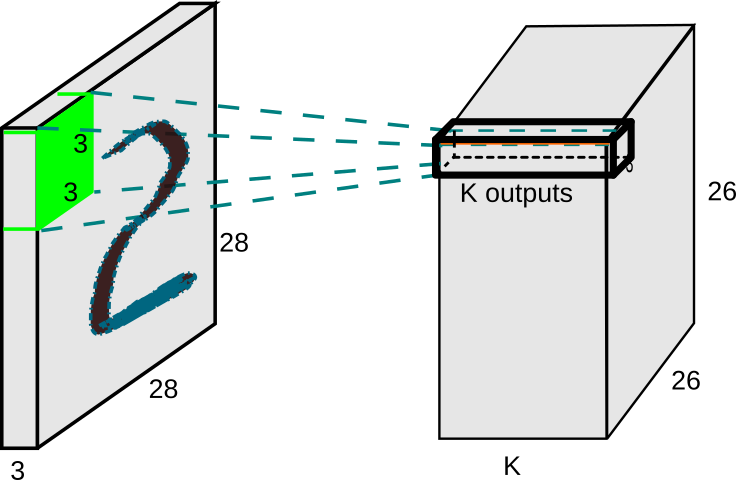
\includegraphics[width=6cm]{img/conv2.png}
\caption{Una vez que la ventana deslizante ha escaneado toda la imagen, se obtiene una matriz tridimensional. Esta matriz tridimensional representa las características aprendidas por la red neuronal durante el proceso de convolución.}
\label{fig: conv2}
\end{figure}

\subsubsection{Ejemplo Convolución}

Supongamos que recibe una imagen de dimensiones $5 \times 5 = 25$ píxeles:

\begin{equation}
	\begin{bmatrix}
	1 & 0 & 1 & 0 & 1 \\
	1 & 1 & 1 & 1 & 0 \\
	0 & 0 & 1 & 1 & 1 \\
	1 & 0 & 0 & 0 & 1 \\
	1 & 1 & 1 & 1 & 1 
	\end{bmatrix}
\end{equation}

\hfill \break
Sea M una red neuronal pequeña de pesos de $3 \times 3$ y una única salida. 
La matríz de pesos es definida para más simplicidad como:

\begin{equation}
	\begin{bmatrix}
	1 & 0 & 1 \\
	0 & 1 & 0 \\
	1 & 0 & 1 
	\end{bmatrix}
\end{equation}

\hfill \break
La matriz resultante de al alimentar la red utilizando la matriz deslizante definida en (2) resulta en el siguiente feature map o mapa de características:

\begin{equation}
	\begin{bmatrix}
	4 & 3 & 5 \\
	3 & 3 & 3 \\
	3 & 3 & 4
	\end{bmatrix}
\end{equation}


\subsubsection{\textbf{Stride \& Padding}}

Corresponden a dos atributos utilizados para controlar el tamaño de los feature maps.

\begin{itemize}
\item	\textit{Stride}: Corresponde a la distancia en la cual se desplaza el núcleo de convolución después de cada aplicación en la matriz de entrada. En otras palabras, determina cuántos píxeles se mueve el filtro o kernel en cada paso de la convolución. Un Stride mayor resulta en una reducción más rápida del tamaño de la salida, mientras que un Stride menor proporciona una salida más detallada.
\item	\textit{Padding}: Se refiere a la cantidad de píxeles que se añaden alrededor del borde de la matriz de entrada antes de aplicar la operación de convolución. Este proceso de ensanchamiento del área de propagación de la matriz deslizante ayuda a preservar la información en los bordes de la imagen. El relleno es útil para evitar la pérdida de información espacial y garantizar que la convolución se aplique de manera uniforme en todas las regiones de la imagen, especialmente en las capas iniciales de la red neuronal convolucional.
\end{itemize}

\subsection{One-Hot Encoding}

En el caso de la representación de objetivos multicategóricos, como en el contexto de imágenes, es esencial emplear un método que permita una representación efectiva de cada categoría para cada imagen. En este sentido, se recurre a la técnica One-Hot Encoding.

Una representación adecuada de One-Hot Encoding es la siguiente.
\setcounter{equation}{0}
\begin{equation}
\mathbf{y} =
\left[ \begin{array}{c} 2 \\ 8 \\ 0 \\ 6 \\ \vdots\end{array} \right]
\Longrightarrow
\begin{bmatrix}
  \textbf{[} 0 & 0 & 1 & 0 & 0 & 0 & 0 & 0 & 0 & 0 \textbf{]} \\
  \textbf{[} 0 & 0 & 0 & 0 & 0 & 0 & 0 & 0 & 1 & 0 \textbf{]} \\
  \textbf{[} 1 & 0 & 0 & 0 & 0 & 0 & 0 & 0 & 0 & 0 \textbf{]} \\
  \textbf{[} 0 & 0 & 0 & 0 & 0 & 0 & 1 & 0 & 0 & 0 \textbf{]} \\
  \vdots & \vdots & \vdots & \vdots & \vdots & \vdots & \vdots & \vdots & \vdots & \vdots
\end{bmatrix}
\end{equation}

En el lado izquierdo, se presenta un vector que contiene etiquetas objetivo en el rango [0, 9]. La matriz del lado derecho corresponde a la representación de cada categoría en una posición del vector, donde el ancho de la matriz se ajusta a la cantidad de categorías (en este caso 10). Cada fila de la matriz representa una instancia de One-Shot Encoding para las respectivas etiquetas objetivo.


\section{Entrenamiento de una CNN}

\subsection{Etapas de una CNN}

Como se mencionó anteriormente, las CNN constan de una serie de etapas. Estas etapas comprenden dos tipos principales de capas: las capas convolucionales y las capas de agrupación (o pooling) (Ver Fig. 2).

\begin{figure}[H]
\centering
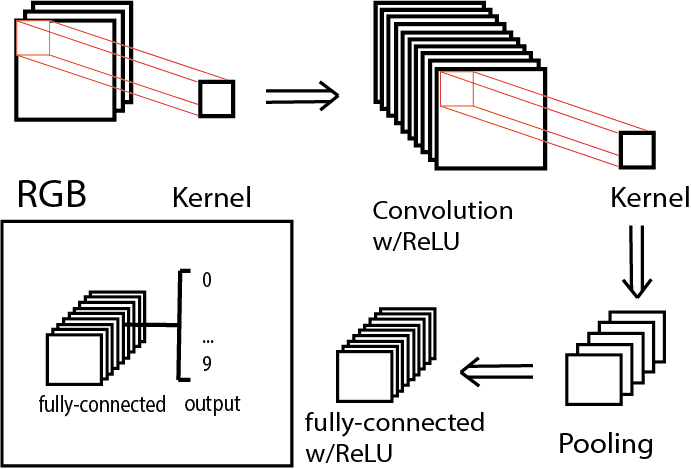
\includegraphics[width=7cm]{img/stagesconv.png}
\caption{En este caso la imagen RGB correspondería a una de dimensiones de MNIST \cite{MNIST}. Las etapas del entrenamiento de una CNN corresponderían a la aplicación de la convolución a las matrices de la imagen, para extraer características relevantes. Posteriormente, la realización de Pooling para reducir la dimensionalidad de la información. Finalmente, la clasificación de la imagen, utilizando las características extraídas por las capas anteriores.}
\label{fig: convpoo}
\end{figure}

\subsection{Hiperparámetros}

\subsubsection{\textbf{Épocas}}

Las épocas corresponden a un ciclo completo de entrenamiento a través de los datos de entrenamiento, lo que permite que la red ajuste sus pesos y mejore su capacidad para hacer predicciones precisas \cite{Epocas}. Este proceso comprende las siguientes etapas:
\begin{itemize}
\item	Foward Propagation: Durante la propagación hacia adelante, los datos de entrenamiento se pasan a través de la red neuronal, capa por capa, desde la entrada hasta la salida. En esta etapa, se calculan las predicciones iniciales de la red en función de los pesos actuales.
\item	Backward Propagation: En esta etapa se calculan las derivadas parciales del error con respecto a los pesos de la red. Estas derivadas se utilizan para ajustar los pesos y mejorar el rendimiento del modelo. 
\end{itemize}

\subsubsection{\textbf{Batch size}}

El hiperparámetro Batch Size se refiere al número de imágenes que se utilizan en la estimación de la gradiente durante el entrenamiento de un modelo. En cada iteración de entrenamiento, el modelo procesa un conjunto de datos de tamaño Batch Size antes de realizar una actualización de los pesos. Según Kandel \cite{BatchSize}, quien se centró en encontrar el valor óptimo de batch para entrenar clasificadores de imágenes, observó que existe una correlación significativa entre la tasa de aprendizaje y el tamaño del batch. En situaciones donde las tasas de aprendizaje son altas, un tamaño de batch grande tiende a desempeñarse mejor que con tasas de aprendizaje bajas. Por lo tanto, sugiere comenzar el entrenamiento de redes neuronales convolucionales (CNN) con un tamaño de batch más pequeño, resaltando la influencia de la relación entre la tasa de aprendizaje y el tamaño del batch en el rendimiento del modelo.


\subsection{Optimizadores}

El optimizador es utilizado para ajustar los pesos de la red con el objetivo de minimizar la función de costo que cuantifica la diferencia entre las predicciones de la RNA y los valores reales. Quiere decir que, por cada época, el optimizador va modificando los pesos sinápticos hasta llegar a una predicción mas cercana a los valores reales que se buscan obtener \cite{Epocas}.

Los optimizadores evaluados utilizados en esta tarea corresponden a Adam \cite{Adam}, Adagrad \cite{Adagrad} y Adadelta \cite{Adadelta}.

\subsubsection{\textbf{Adam}} Se trata de un algoritmo de optimización estocástica que combina las ventajas de dos métodos de optimización recientemente populares: la capacidad de AdaGrad para manejar gradientes dispersos y la habilidad de RMSProp para lidiar con objetivos no estacionarios.

\subsubsection{\textbf{Adadelta}} Este método presenta la particularidad de no requerir ajustes manuales en la tasa de aprendizaje, mostrándose robusto frente a la presencia de información de gradientes ruidosa, diferentes elecciones de arquitectura de modelos, diversas modalidades de datos y la selección de hiperparámetros. Los resultados prometedores obtenidos en comparación con otros métodos, tanto en tareas de clasificación de dígitos MNIST en una sola máquina como en conjuntos de datos vocales a gran escala en entornos de clúster distribuido, respaldan la eficacia de Adadelta y demuestran la útilidad de este en la tarea.

\subsubsection{\textbf{Adagrad}} Adagrad, un método adaptativo de subgradiente, se presenta como una herramienta que ajusta los métodos de subgradiente según la geometría específica del problema. Esta adaptación asegura garantías sólidas de arrepentimiento, superando en rendimiento a algoritmos anteriores en algunas distribuciones naturales de datos. Al adaptarse a la geometría específica del problema, Adagrad permite realizar ajustes más precisos en parámetros que experimentan gradientes más escasos o frecuentes.

\section{Bases de Datos}

Para el entrenamiento adecuado de la Red Neuronal Convolucional CNN es requerido un buen repertorio de bases de datos. En este caso, se escogieron MNIST \cite{MNIST} y CIFAR-10 \cite{CIFAR10} debido a la gran contribución que han entregado a todas las investigaciones relacionadas con CNN. Estas bases de datos fueron cuidadosamente creadas para proporcionar una variedad representativa de imágenes que abarcan desde dígitos escritos a mano hasta objetos cotidianos en diferentes escenarios. 

\subsection{MNIST}

La base de datos MNIST (Modified National Institute of Standards and Technology database) es un problema de clasificación multiclase en el que se nos pide que clasifiquemos un dígito ($0-9$) a partir de una imagen en escala de grises de $28\times 28$:
Este contiene 60000 ejemplos y un conjunto de prueba con 10000 ejemplos. Estos digitos tienen un tamaño normalizado y centrado se encuentran en una imagen de tamaño fijo. Originalmente, las imágenes en blanco y negro del NIST se normalizaron de tamaño para ajustarse a un cuadro de píxeles de $20 \times 20$, preservando su relación de aspecto. Las imágenes resultantes contienen niveles de gris debido a la técnica de antialiasing utilizada por el algoritmo de normalización. Luego, las imágenes se centraron en un campo de $28 \times 28$ al calcular el centro de masa de los píxeles y traducir la imagen para posicionar este punto en el centro del campo de $28 \times 28$.

\subsection{CIFAR10}

El conjunto de datos CIFAR-10 consta de 60000 imágenes a color de $32 \times 32$ píxeles distribuidas en 10 clases (Ver Fig. 3), con 6000 imágenes por clase. Se compone de 50000 imágenes de entrenamiento y 10000 imágenes de prueba.

Este conjunto de datos se divide en cinco lotes de entrenamiento y un lote de prueba, cada uno con 10000 imágenes. El lote de prueba contiene exactamente 1000 imágenes seleccionadas aleatoriamente de cada clase. Los lotes de entrenamiento contienen las imágenes restantes en un orden aleatorio, aunque algunos lotes de entrenamiento pueden contener más imágenes de una clase que de otra. En conjunto, los lotes de entrenamiento contienen exactamente 5000 imágenes de cada clase.

\begin{figure}[H]
\centering
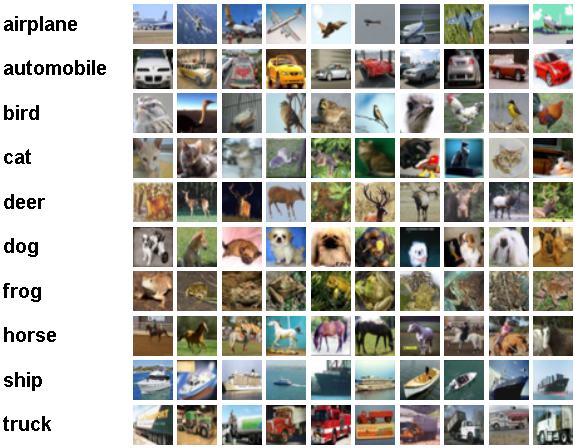
\includegraphics[width=6cm]{img/CIFAR10.png}
\caption{Diferentes muestras de imágenes correspondientes a una de las 10 clases disponibles en el conjunto de datos CIFAR-10.}
\label{fig}
\end{figure}

\section{Metodología}

\subsection{Herramientas}

El entrenamiento de las CNN se llevó a cabo en el entorno de Google Colab, utilizando las librerías TensorFlow y Keras con el lenguaje de programación Python para una implementación más sencilla. Se emplearon los conjuntos de datos MNIST y CIFAR-10 tanto para el entrenamiento como para la evaluación de los modelos de CNN.

\subsubsection{\textbf{MNIST}}

En principio, el enfoque corresponde a entrenar la Red Neuronal Convolucional (CNN) con el conjunto de datos MNIST que se importaron en el código mediante Keras.

Se tiene que el conjunto de datos entregados por Keras tiene las siguientes dimensiones para el conjunto de entrenamiento y prueba:

\begin{itemize}
\item	Shape of x\_train (60000, 28, 28)
\item	Shape of y\_train (60000,)
\item	Shape of x\_test (10000, 28, 28)
\item	Shape of y\_test (10000,)
\end{itemize}

\begin{figure}[h!]
\centering
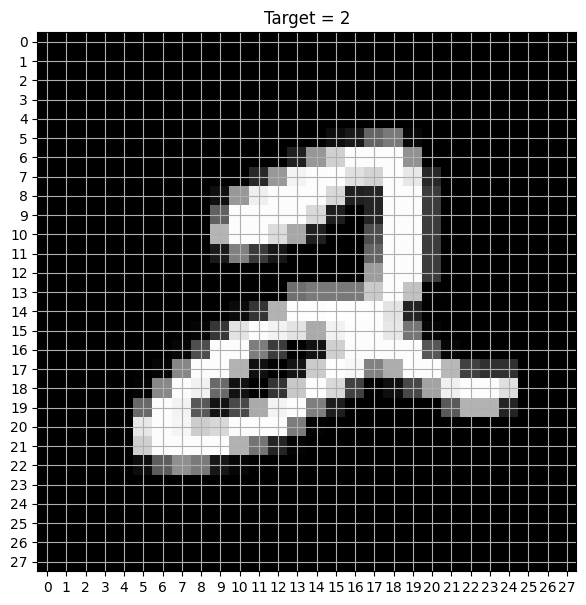
\includegraphics[width=6cm]{img/mnist1.png}
\caption{Corresponde a la 5ta muestra obtenida luego de cargar la base de datos MNIST.}
\label{fig: mnist1}
\end{figure}

\subsection{Preprocesamiento de datos}

El primer paso corresponde a realizar un sistema que permita la normalización de las imágenes mediante alguna función. Esta debe normalizar las imágenes de 8 bits de [0, 255] a flotantes de [0,1].

Como estamos tratando con imágenes bastaría con:

\begin{equation}
f(x) = \frac{x}{255}
\end{equation}

\begin{itemize}
\item	x es un valor de la imagen RGB.
\item	f(x) es el valor de la imagen RGB dividido por 255.
\end{itemize}

\subsubsection{\textbf{Ampliar la dimensión de entrada}}

Debido a que las operaciones de convolución se realizan sobre los canales de color de la imagen, una imagen en escala de grises necesitaría un canal adicional de color para poder entrenar los modelos y es por ello que se agrega una dimensión más a las imágenes. Para este fin, se utilizón la función de numpy: expand\_dims (Ver Fig. 5).


\begin{figure}[h!]
\centering
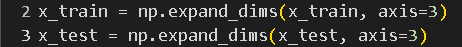
\includegraphics[width=8cm]{img/dims.png}
\caption{Corresponde a un fragmento de código en el que utiliza la función expand\_dims de numpy.}
\label{fig: dims}
\end{figure}

\subsubsection{\textbf{Función para One-Shot Encoding}}

\setcounter{equation}{0}
\begin{flalign*}
\hline
&\text{\textbf{Function}} \quad one\_hot \quad \text{\textbf{Params}} \leftarrow (vector, number\_classes) \\
&\quad one\_hot  \leftarrow empty\_array \\
&\quad \text{\textbf{For}} \quad i \leftarrow vector ++\\
&\quad \quad aux \leftarrow \text{zeros[length(number\_classes)]} \\
&\quad \quad aux[i] = 1 \\
&\quad \quad one\_hot \leftarrow aux \\
&\quad \text{\textbf{Endfor}} \\
&\text{\textbf{Endfunction}} \\
\hline
\end{flalign*}

\subsection{Implementación de Red Neuronal Convolucional}

Se implementan  2 CNN, una llamada net\_1() (Ver Fig. 6) ubicada en una función que recibe el tamaño de las muestras y la cantidad de clases. Esta contiene la arquitectura de la CNN donde se adecua mediante la función Input de keras.layers las dimensiones de las entradas y las conexiones internas mediante Conv2D de keras.layers donde se especifica el uso de función de activación ReLU y una cantidad de zero-padding (Ver Fig. 8).


\begin{figure}[h!]
\centering
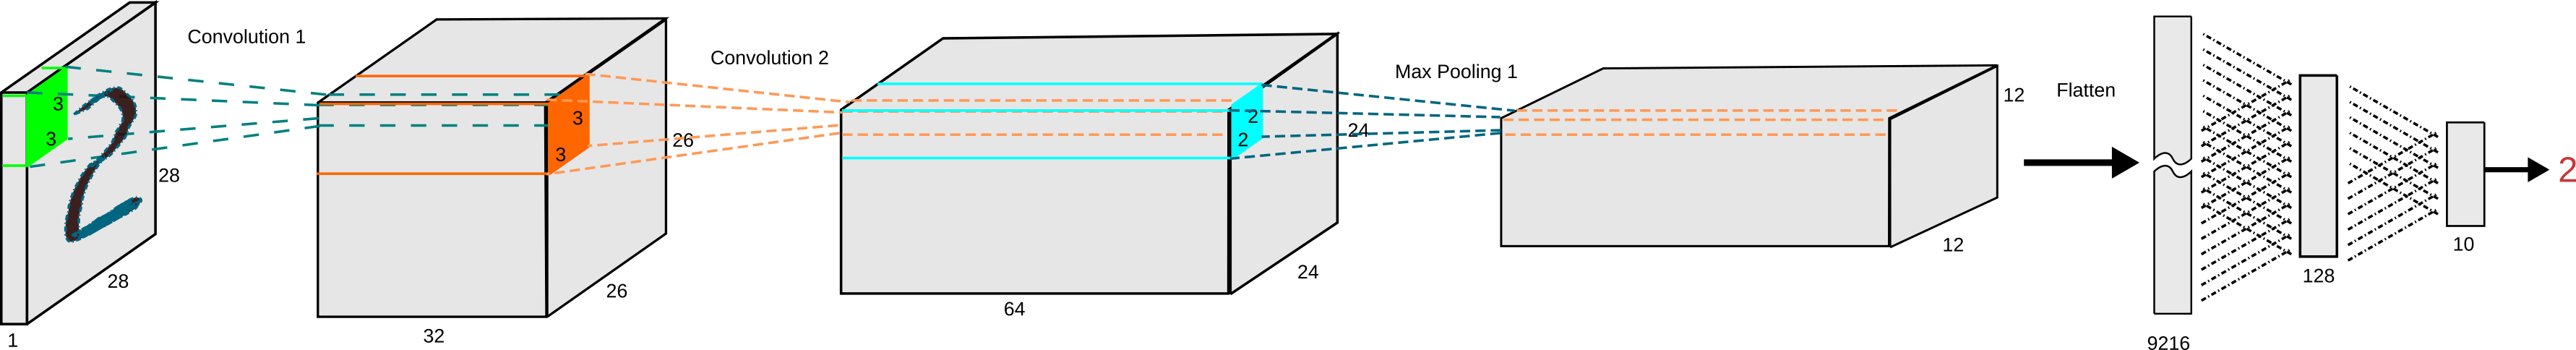
\includegraphics[width=8cm]{img/net1.png}
\caption{Corresponde a una representación visual del modelo net\_1 implementado.}
\label{fig: net1}
\end{figure}

\begin{figure}[h!]
\centering
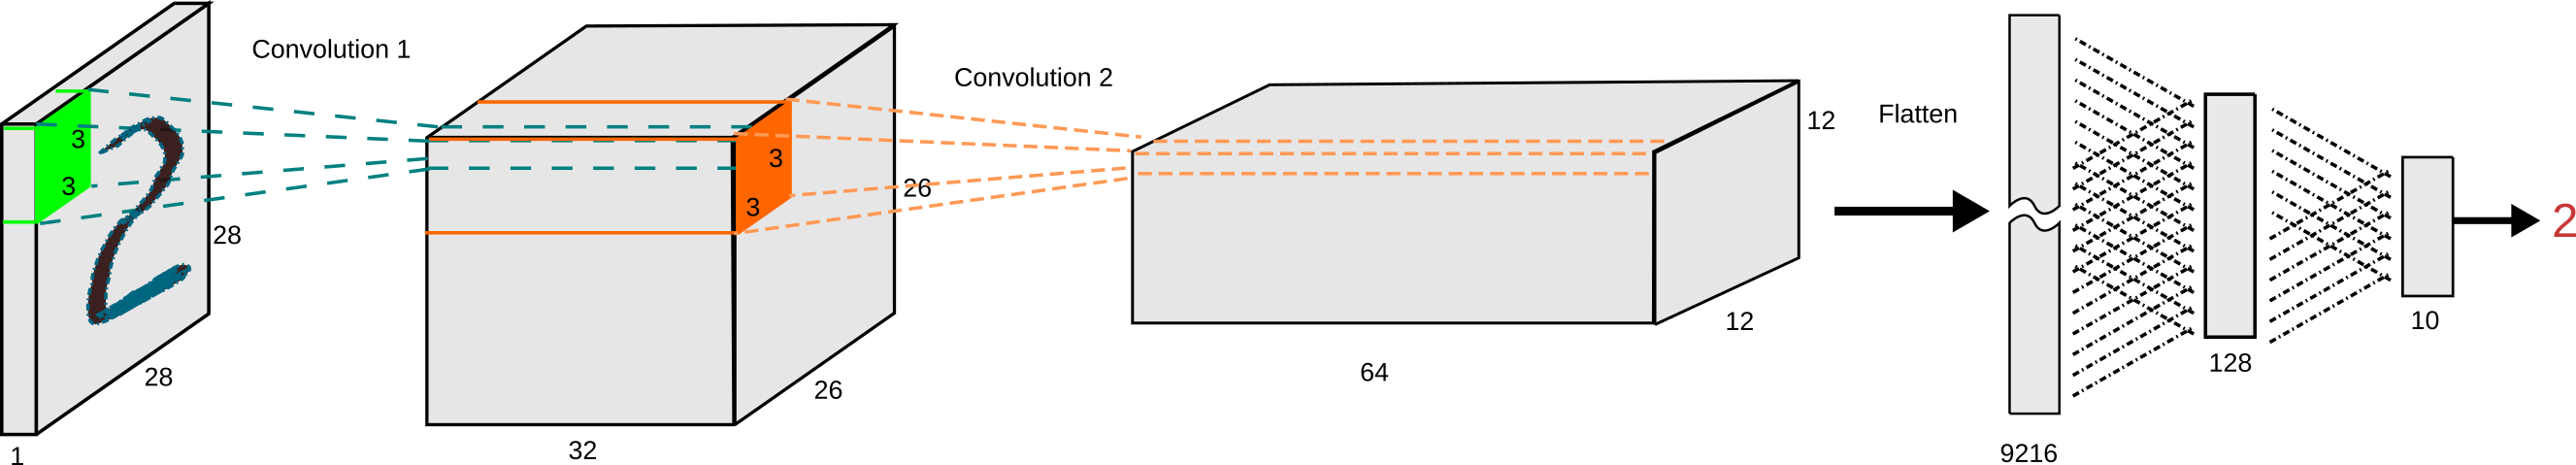
\includegraphics[width=8cm]{img/net2.png}
\caption{Corresponde a una representación visual del modelo net\_2 implementado.}
\label{fig: net2}
\end{figure}


Luego se agrega el uso de MaxPooling con MaxPooling2D de keras.layers que tendrá una dimensión de $2 \times 2$ y zero-padding. La implementación continúa con la operación de aplanado (Flatten) para transformar los datos en un formato unidimensional, seguido de una capa completamente conectada (Dense) con 128 unidades y activación ReLU. Finalmente, se agrega otra capa densa con la función de activación softmax para obtener las probabilidades de pertenencia a cada clase.
Para la segunda CNN llamada net\_2() (Ver Fig. 9) se removió la capa de max pooling y se añadió un stride de valor 2 al segundo bloque de la convolución.

\begin{figure}[h!]
\centering
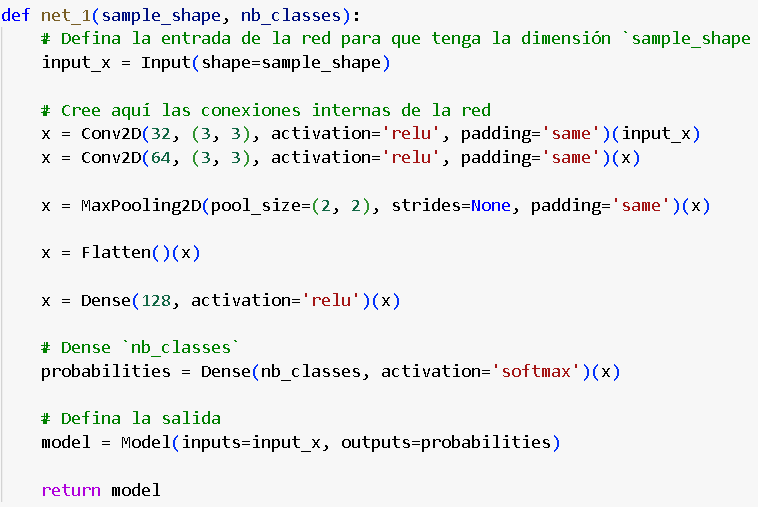
\includegraphics[width=8.5cm]{img/codenet1.png}
\caption{Implementación de función net\_1 que contiene el diseño de la arquitectura de la Red Neuronal Convolucional.}
\label{fig: codenet1}
\end{figure}

\begin{figure}[h!]
\centering
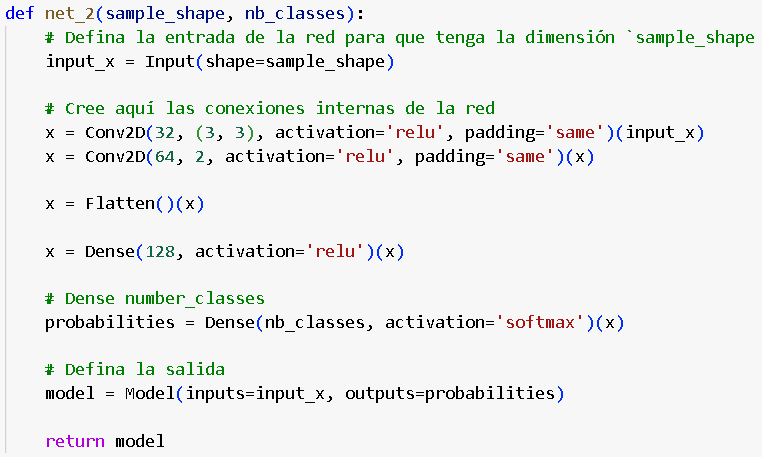
\includegraphics[width=8.5cm]{img/codenet2.png}
\caption{Implementación de función net\_2 que contiene el diseño de la arquitectura de la Red Neuronal Convolucional sin la implementación de MaxPooling.}
\label{fig: codenet2}
\end{figure}

\subsection{Definición de Hiperparámetros}

Se implementó un Early Stopping similar al de la Tarea N2 \cite{Epocas} para encontrar los mejores hiperparamétros batch y épocas para este tipo de redes. Se descubrió que basta con los valores anteriormente recomendados por Kandel \cite{BatchSize} para el batch correspondiente a valores de 32 a 40 y una cantidad de épocas mayor a 280 para el término del entrenamiento. Para esta función de Early Stopping es importante mencionar que se utilizó el Optimizador Adadelta, por lo que seguramente aplicando Adagrad o Adam termine antes o demore más y consuma aún más recursos.

\section{Resultados MNIST}

Se realiza el entrenamiento de los modelos con los diseños net\_1 y net\_2 explicados previamente y el conjunto de datos MNIST con el principal objetivo de comparar rendimientos entre net\_1 y net\_2 puesto que difieren de la implementación de Max Pooling.
\hfill\break
\subsection{Entrenamiento net\_1}

Se realiza una compilación del modelo definido con la arquitectura net\_1 y posteriormente se entrena con la función \textit{fit}, la cual recibe los conjuntos de entrenamiento, los hiperparámetros \textit{batch} y \textit{épocas}, el tipo de display con \textit{verbose} y el \textit{validation\_split}, que define el porcentaje del conjunto para validación.

\hfill\break
Epoch 41/45\\
1543/1543 - 7s - loss: 0.2118 - accuracy: 0.9393 - val\_loss: 0.1670 - val\_accuracy: 0.9535 - 7s/epoch - 5ms/step\\
Epoch 42/45\\
1543/1543 - 7s - loss: 0.2092 - accuracy: 0.9400 - val\_loss: 0.1665 - val\_accuracy: 0.9528 - 7s/epoch - 5ms/step\\
Epoch 43/45\\
1543/1543 - 7s - loss: 0.2066 - accuracy: 0.9406 - val\_loss: 0.1638 - val\_accuracy: 0.9550 - 7s/epoch - 4ms/step\\
Epoch 44/45\\
1543/1543 - 7s - loss: 0.2043 - accuracy: 0.9416 - val\_loss: 0.1618 - val\_accuracy: 0.9555 - 7s/epoch - 5ms/step\\
Epoch 45/45\\
1543/1543 - 6s - loss: 0.2018 - accuracy: 0.9418 - val\_loss: 0.1598 - val\_accuracy: 0.9568 - 6s/epoch - 4ms/step\\

\begin{figure}[h!]
\centering
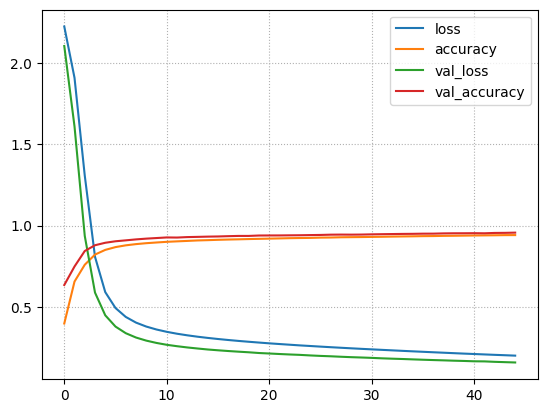
\includegraphics[width=7cm]{img/definiryentrenar1.png}
\caption{Resultados del entrenamiento del modelo definido con la función net\_1 con esto se concluye que para el optimizador Adadelta un batch de 35 y una cantidad de épocas mayores a 280 convergen a valores más pequeños para loss y val\_loss.}
\label{fig: definiryentrenar1}
\end{figure}

\subsection{Entrenamiento net\_2}

Al igual que con net\_1, se entrena el modelo definido con la arquitectura net\_2, esto con el fin de analizar los efectos del entrenamiento sin Max Pooling y al igual que con net\_1 se realiza una compilación del modelo y se procede a entrenarlo utilizando la función \textit{fit}. 

Los siguientes corresponden a los valores de las últimas épocas:

\hfill\break
Epoch 41/45\\
1543/1543 - 8s - loss: 0.1785 - accuracy: 0.9485 - val\_loss: 0.1465 - val\_accuracy: 0.9613 - 8s/epoch - 5ms/step\\
Epoch 42/45\\
1543/1543 - 8s - loss: 0.1761 - accuracy: 0.9494 - val\_loss: 0.1449 - val\_accuracy: 0.9618 - 8s/epoch - 5ms/step\\
Epoch 43/45\\
1543/1543 - 8s - loss: 0.1739 - accuracy: 0.9500 - val\_loss: 0.1434 - val\_accuracy: 0.9617 - 8s/epoch - 5ms/step\\
Epoch 44/45\\
1543/1543 - 8s - loss: 0.1717 - accuracy: 0.9501 - val\_loss: 0.1415 - val\_accuracy: 0.9628 - 8s/epoch - 5ms/step\\
Epoch 45/45\\
1543/1543 - 8s - loss: 0.1696 - accuracy: 0.9510 - val\_loss: 0.1401 - val\_accuracy: 0.9632 - 8s/epoch - 5ms/step\\

\begin{figure}[h!]
\centering
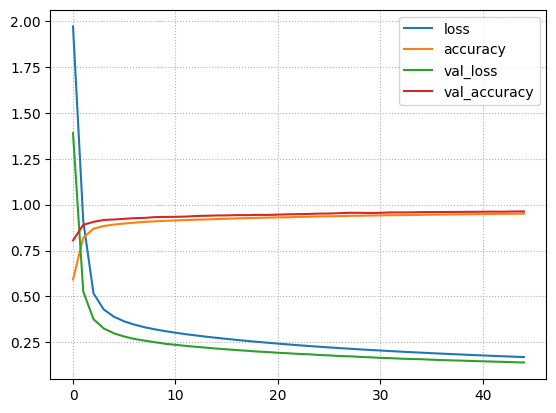
\includegraphics[width=7cm]{img/definiryentrenar2.png}
\caption{Resultados del entrenamiento del modelo definido con la función net\_2. Muestran que sin Max Pooling se tiene un rendimiento que compite con net\_1, aunque es algo más lento.}
\label{fig: definiryentrenar1}
\end{figure}

\section{Resultados CIFAR-10}

En la investigación sobre el rendimiento de las Redes Neuronales Convolucionales entrenadas con CIFAR-10, se llevó a cabo el proceso de entrenamiento (fitting) utilizando los modelos definidos por las arquitecturas net\_1 y net\_2. Además, se realizaron evaluaciones utilizando tres optimizadores distintos: Adam, Adadelta y Adagrad. Esta elección se fundamenta en la complejidad de las imágenes presentes en CIFAR-10, lo que permite analizar y comparar el rendimiento de los modelos con estos optimizadores en condiciones desafiantes.
\hfill\break
\subsection{Entrenamiento net\_1}

Se definen 3 modelos para los 3 optimizadores disponibles y se cambiaron los hiperparámetros a una cantidad de épocas de 30 y batch de tamaño 128. Además, se aumenta el tamaño del conjunto de validación cambiando el parámetro de validation\_split de 0.1 a 0.2.

Se muestran a continuación las épocas con mejores resultados para cada uno de los optimizadores y las gráficas correspondientes.

\subsubsection{\textbf{Adadelta} (Ver Fig. 12)} 
\hfill\break
Epoch 30/30\\
352/352 - 3s - loss: 1.8676 - accuracy: 0.3614 - val\_loss: 1.8768 - val\_accuracy: 0.3516 - 3s/epoch - 10ms/step

\begin{figure}[h!]
\centering
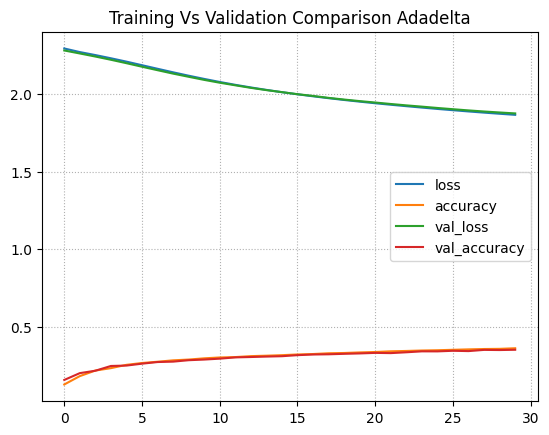
\includegraphics[width=6cm]{img/net1adadelta.png}
\caption{Adadelta tiene poco accuracy y un alto val\_loss en la época 30 y complementando con la gráfica se estima que tiene mayor potencial a mayor cantidad de épocas al usar batch de 128.}
\label{fig: net1adadelta}
\end{figure}

\subsubsection{\textbf{Adagrad} (Ver Fig. 13)} 
\hfill\break
Epoch 30/30\\
352/352 - 3s - loss: 1.3897 - accuracy: 0.5162 - val\_loss: 1.4119 - val\_accuracy: 0.5090 - 3s/epoch - 9ms/step

\begin{figure}[h!]
\centering
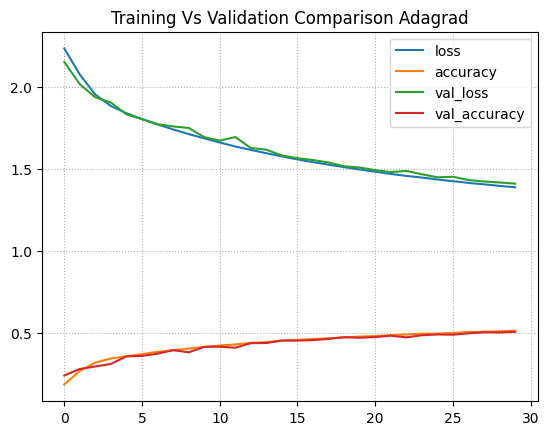
\includegraphics[width=6cm]{img/net1adagrad.png}
\caption{Adagrad tiene un accuracy de 0.51 y un alto val\_loss en la época 30 y complementando con la gráfica se estima que tiene mayor potencial a mayor cantidad de épocas al usar batch de 128, pero además presenta un poco de overfitting.}
\label{fig: net1adagrad}
\end{figure}

\subsubsection{\textbf{Adam} (Ver Fig. 14)} 
\hfill\break
Epoch 4/30\\
352/352 - 4s - loss: 0.7562 - accuracy: 0.7388 - val\_loss: 0.8931 - val\_accuracy: 0.6982 - 4s/epoch - 10ms/step

\begin{figure}[h!]
\centering
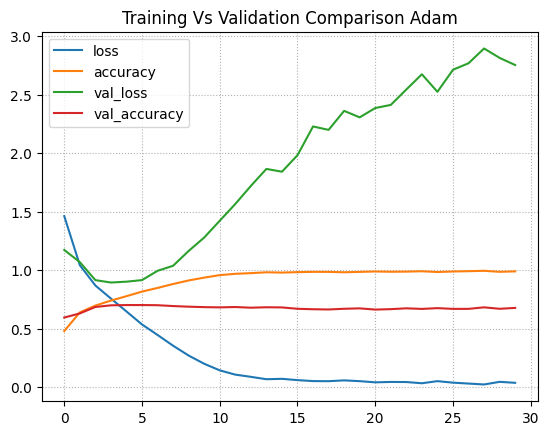
\includegraphics[width=6cm]{img/net1adam.png}
\caption{Adam tiene un accuracy de 0.73 y un alto val\_loss en la época 4, pero posterior a eso aumenta el valor de val\_loss y el accuracy dando como evidencia de que tiene un sobreajuste bastante grande.}
\label{fig: net1adam}
\end{figure}

\subsection{Entrenamiento net\_2}

Se realiza el mismo procedimiento para los modelos con net\_2. Se muestran a continuación las épocas con mejores resultados para cada optimizador:

\subsubsection{\textbf{Adadelta} (Ver Fig. 15)} 
\hfill\break
Epoch 30/30\\
352/352 - 4s - loss: 1.7560 - accuracy: 0.3978 - val\_loss: 1.7703 - val\_accuracy: 0.3904 - 4s/epoch - 12ms/step

\begin{figure}[h!]
\centering
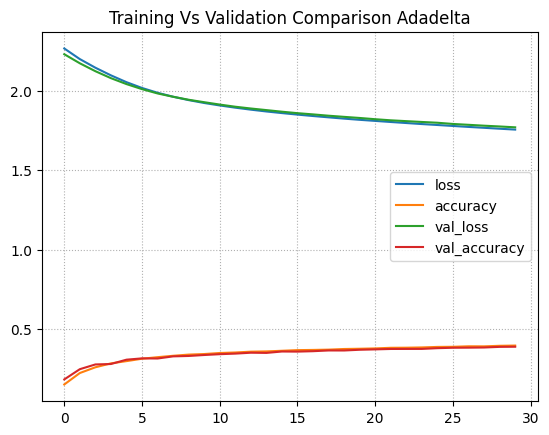
\includegraphics[width=6cm]{img/net2adadelta.png}
\caption{Muestra el progreso de las variables loss, accuracy, val\_los y val\_accuracy através de las épocas para el modelo net\_2 con el optimizador Adadelta.}
\label{fig: net2adadelta}
\end{figure}

\subsubsection{\textbf{Adagrad} (Ver Fig. 16)} 
\hfill\break
Epoch 29/30\\
352/352 - 4s - loss: 1.3876 - accuracy: 0.5153 - val\_loss: 1.4161 - val\_accuracy: 0.5098 - 4s/epoch - 11ms/step\\
Epoch 30/30\\
352/352 - 4s - loss: 1.3780 - accuracy: 0.5200 - val\_loss: 1.4438 - val\_accuracy: 0.4872 - 4s/epoch - 11ms/step

\begin{figure}[h!]
\centering
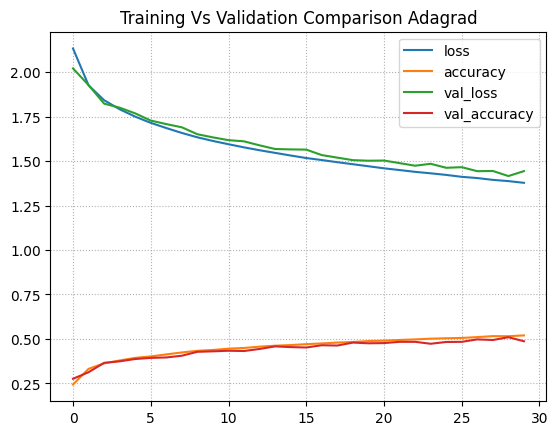
\includegraphics[width=6cm]{img/net2adagrad.png}
\caption{Muestra el progreso de las variables loss, accuracy, val\_los y val\_accuracy através de las épocas para el modelo net\_2 con el optimizador Adagrad.}
\label{fig: net2adagrad}
\end{figure}

\subsubsection{\textbf{Adam} (Ver Fig. 17)} 
\hfill\break
Epoch 5/30\\
352/352 - 4s - loss: 0.6796 - accuracy: 0.7654 - val\_loss: 1.0173 - val\_accuracy: 0.6548 - 4s/epoch - 11ms/step

\begin{figure}[h!]
\centering
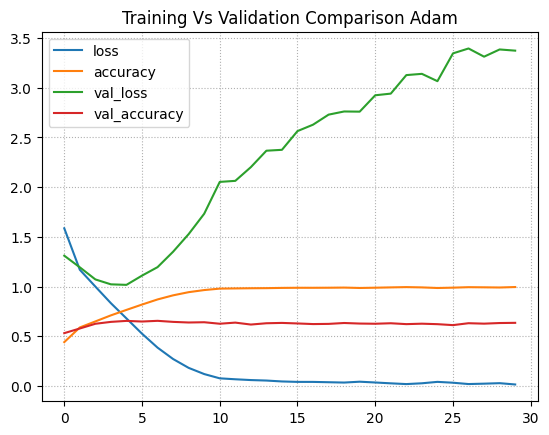
\includegraphics[width=6cm]{img/net2adam.png}
\caption{Muestra el progreso de las variables loss, accuracy, val\_los y val\_accuracy através de las épocas para el modelo net\_2 con el optimizador Adam.}
\label{fig: net2adam}
\end{figure}

\section{Análisis}

\subsection{Resultados MNIST}

Se puede observar que tanto el modelo definido por la arquitectura net\_1 con Max Pooling como net\_2 sin la implementación de este, demuestran un buen rendimiento y potencial en el entrenamiento con conjuntos de datos menos complejos, como MNIST, que contiene dígitos hechos a mano en escala de grises. Este rendimiento se refleja en los resultados obtenidos en las épocas, donde ambos modelos muestran en la época 45 un val\_loss de 0.1598 en net\_1 con una tardanza de 6 segundos por época y 0.1401 en net\_2 con una tardanza de 8 segundos por época corroborado con las gráficas de Fig. 10 y Fig. 11 que muestran que la convergencia es limpia. Este comportamiento puede deberse, en parte, al uso del optimizador Adadelta, que contribuye a una convergencia más eficiente y a la prevención del sobreajuste.

\subsection{Resultados CIFAR-10}

Una vez obtenidos los resultados del entrenamiento de los modelos net\_1 y net\_2 con el conjunto de datos CIFAR y los 3 optimizadores se pueden obtener las siguientes afirmaciones:
\hfill\break
\subsubsection{\textbf{Modelo de mejor funcionamiento}}

Con los resultados obtenidos del conjunto de datos con imágenes más complejas se puede comprobar que el modelo que mejor funciona corresponde a net\_1 debido principalmente a la evolución de las variables loss, val\_loss, accuracy y val\_accuracy  vistos en Fig. 12, Fig. 13 y Fig 14 mostrando que existe una menor cantidad de ruido al momento de entrenar a diferencia de net\_2 que no utiliza Max Pooling. Este ruido es peligroso puesto que es signo de un futuro sobreajuste en el entrenamiento esto también evidenciado de mejor manera después de entrenar el modelo net\_1 y net\_2 con el optimizador Adam.

\subsubsection{\textbf{Optimizador de mejor funcionamiento}}

En los entrenamientos realizados con los conjuntos de datos MNIST y CIFAR-10, se observó que Adadelta proporciona una convergencia más eficiente y superior en ambos modelos, net\_1 y net\_2, en comparación con los otros optimizadores. Esta tendencia es evidente en las figuras Fig. 12 a Fig. 17, donde Adadelta exhibe un mayor potencial y menor ruido, sugiriendo que podría permitir un entrenamiento más prolongado con un rendimiento continuo.

\subsubsection{\textbf{Overfitting}}
En el caso del optimizador Adagrad, se observa una tendencia hacia un posible sobreajuste futuro, atribuible a la presencia de un nivel significativo de ruido en la convergencia, particularmente evidente en los modelos net\_1 y net\_2.

En cuanto al optimizador Adam, se detecta un sobreajuste evidente después de la época 4 con el modelo net\_1 y después de la época 5 con el modelo net\_2. En estas instancias, el modelo ajusta excesivamente sus parámetros a los datos de entrenamiento, mostrando una falta de generalización a nuevos datos.

\subsubsection{\textbf{Rendimiento}}

El rendimiento a largo plazo se vuelve más plausible con la implementación de Adadelta y un modelo con la arquitectura net\_1 utilizando Max Pooling, como se evidencia en los resultados presentados. Por lo tanto, se podría observar una mejora significativa en el rendimiento al permitir que el modelo net\_1 continúe entrenándose en un entorno con recursos computacionales adecuados. Es importante tener en cuenta que, en un entorno básico de Colab, se limita a un máximo de 280 épocas. Además, se sugiere aplicar la técnica de detención temprana (Early Stopping) para optimizar el entrenamiento.


\section{Conclusiones generales}

Esta tarea proporciona una visión detallada del rendimiento de las Redes Neuronales Convolucionales (CNN) en conjuntos de datos de diversa complejidad y bajo las diferentes arquitecturas Adam, Adadelta y Adagrad. 
\hfill\break
Los resultados sugieren que la elección del optimizador y la arquitectura puede tener un impacto significativo en la convergencia y el rendimiento a largo plazo de las redes neuronales.
\hfill\break
Se destaca la eficacia del optimizador Adadelta y la importancia de considerar cuidadosamente la implementación de capas como Max Pooling en la arquitectura de la red. 
\hfill\break
Finalmente, se sugiere que, para obtener resultados más significativos, se permita que el modelo net\_1 continúe entrenándose en un entorno con recursos computacionales adecuados. Además, se recomienda la aplicación de la técnica de detención temprana (Early Stopping) para evitar el sobreajuste.

\section*{Bibliografía}
\def\refname{}
\begin{thebibliography}{34}
	\bibitem{CNN} LeCun, Y., Bengio, Y., \& Hinton, G. (2015). Deep learning. Nature, 521(7553), 436–444. doi:10.1038/nature14539 
	
	\bibitem{MNIST} LeCun, Yann and Cortes, Corinna and Burges, CJ. (2010). MNIST handwritten digit database, ATT Labs [Online] Volume 2. Available: \url{http://yann.lecun.com/exdb/mnist}
	\url{https://paperswithcode.com/dataset/mnist}
	
	\bibitem{CIFAR10} Krizhevsky, A. (2009). Learning Multiple Layers of Features from Tiny Images. \\ \url{https://www.cs.toronto.edu/~kriz/cifar.html}
	
	\bibitem{ONESHOT} Michael Guerzhoy (2016). CSC321: Intro to Machine Learning and Neural Networks. \\ \url{https://www.cs.toronto.edu/~guerzhoy/321/lec/W04/onehot.pdf}
	
	\bibitem{BatchSize} I. Kandel and M. Castelli, The effect of batch size on the generalizability of the convolutional neural networks on a histopathology dataset, ICT Express (2020),
https://doi.org/10.1016/j.icte.2020.04.010.
	
	\bibitem{Epocas} Araya, N., Bugueño, I. (2023) Tarea N2: Redes Neuronales
\url{https://github.com/NicolasAraya932/IAHOMEWORK/blob/main/InformeTarea2IANicolasAraya.pdf}

	\bibitem{IntroCNN} O'Shea, K., \& Nash, R. (2015). An Introduction to Convolutional Neural Networks. arXiv:1511.08458
	
	\bibitem{Adam} Diederik, P. Kingma \& Jimmy, Ba. (2017). Adam: A Method for Stochastic Optimization. arXiv:1412.6980
	
	\bibitem{Adagrad} Duchi, J., Hazan, E., \& Singer, Y. (2011). Adaptive Subgradient Methods for Online Learning and Stochastic Optimization. (T. Zhang, Ed.). Journal of Machine Learning Research 12 (2011) 2121-2159, 12. 
	
	\bibitem{Adadelta} Matthew D. Zeiler. (2012). ADADELTA: An Adaptive Learning Rate Method. arXiv:1212.5701
	
	\bibitem{DNN} Huang Yi, Sun Shiyu, Duan Xiusheng, \& Chen Zhigang. (2016). A study on Deep Neural Networks framework. 2016 IEEE Advanced Information Management, Communicates, Electronic and Automation Control Conference (IMCEC). doi:10.1109/imcec.2016.7867471
\end{thebibliography}

\end{document}
